\section{Andmestiku loomine}
Käesolevas osas käsitletakse andmestiku loomise protsessi, sealhulgas andmete kogumist, töötlemist ja maskimist. Andmestiku loomine on oluline samm igasuguste andmete analüüsimisel ja seda ka masinõppe projektide puhul. Andmete kvaliteet ja sobivus mõjutavad otseselt mudeli täpsust ja usaldusväärsust. Nagu muudes valdkondades kehtib ka informaatikas Pareto printsiip, mille kohaselt 80\% probleemidest tuleneb 20\% põhjustest. Seega on andmestiku loomine ja töötlemine äärmiselt oluline etapp, mis võib määrata kogu projekti edasise käigu.

\subsection{Raie piirkonna andmete kogumine}
Metsateatis on dokument, mille kaudu metsaomanik esitab Keskkonnaametile
kavandatavate raietööde või oluliste metsakahjustuste kohta teabe. Keskkonnaamet
kontrollib esitatud teatiste nõuetekohasust ning veendub, et kavandatav raie
vastab kehtivatele õigusaktidele. Metsateatised menetletakse ja säilitatakse
riiklikus metsaregistris. Peale edukat menetlemist võib raietöödega alustada 10 päeva peale otsust ja kuni 24 kuu jooksul. \cite{MetsateatisJaMetsaregister} Metsateatised on avalikud ja neid saab vaadata riiklikus metsaregistris.

Metsade inventeerimise ja registrisse kandmise protsess algab metsaeraldiste
täpse kaardistamisega, kasutades L‑EST97 ristkoordinaatide süsteemi, Eesti
põhikaarti, katastriüksuse plaane ning vajadusel kaugseire andmeid eraldiste
piiritlemiseks ja võimalike situatsioonielementide täpsustamiseks. Kaardistamise
tulemusena koostatakse geoinfosüsteemi metsaeraldiste kiht, kus iga eraldis on
nummerdatud ning selle pindala, arvutatuna piiripunktide koordinaatide alusel, 
esitatakse hektarites vähemalt kümnendkohani ning täpsusega 10 meetrit --- see
loob aluse usaldusväärsele pindalaarvestusele ja edaspidistele
takseerimistoimingutele. \cite{MetsaKorraldamiseJuhend}

Koostöös Keskkonnaagentuuriga saadi andmed metsateatistest, mis sisaldavad teavet nii metsateatise esitamise kuupäeva, metsateatise menetlemise kuupäeva, metsateatise kehtivuse alguskuupäeva kui ka metsateatise kehtivuse lõppkuupäeva kohta. Kuna riigimetsade teatised on täpsemas seisukorras, siis võeti need raieteatised selle uurimustöö aluseks. Seoses sellega et ühe lõigu peal võib olla väga väike kogus metsa, sai teatiste pärimine ümber ehitatud sedasi, et ühe metsa raie ümber kogutakse peale raie toimumist kokku ka kõik teiste raiete raadiuses asuvad piirkonnad, millel on teada, kas on mets või raieala. Piirkonniti pärimine sai teostatud kasutades PostGISi liidest Postgresi andmebaasiga. Iga raie sisaldab ka endas geomeetria veergu, mis esitab polügooni kujul selle asukohta. 

Polügoon ehk hulknurk on geomeetriline kujund, mis määratleb kindla ala, ühendades üksteisega
punktid, et moodustada suletud piirjoon. Andmetöötluse ja ruumiandmete analüüsi
kontekstis kasutatakse polügoone, et täpselt määratleda geograafilisi alasid. \cite{WhatLocationPolygon}


\begin{figure}[H]
    \centering
    \hspace{-0.5cm}\subfloat[]{{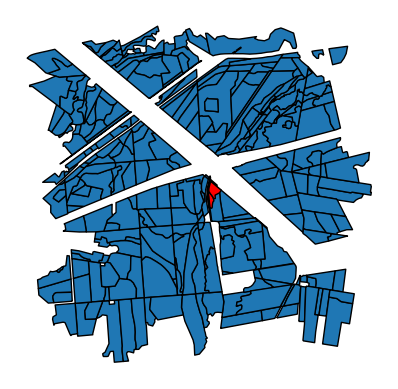
\includegraphics[width=0.5\textwidth]{figures/andmestik/er_id_is_3308099.png}
    	}}
    %\begin{subfigure}[b]{0.5\textwidth} % Set width for side-by-side arrangement
    %    \centering
    %    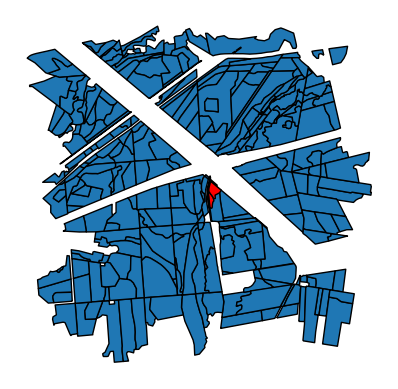
\includegraphics[width=0.5\textwidth]{figures/andmestik/er_id_is_3308099.png}
    %    \caption{}
    %    \label{fig:umbrusexample}
    %\end{subfigure}
    %% Second subfigure
    \subfloat[]{{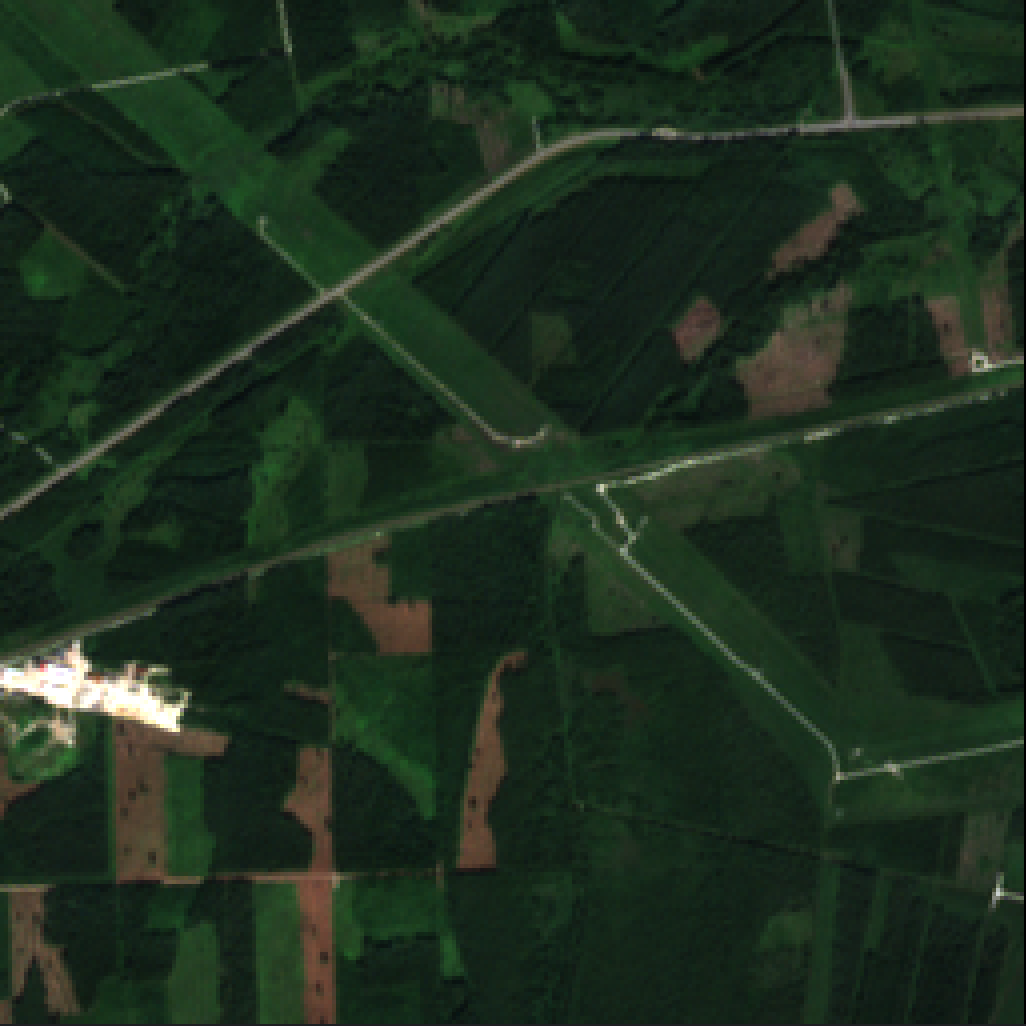
\includegraphics[width=0.5\textwidth]{figures/andmestik/lr_3308099_TCI.png}
}}

    %\begin{subfigure}{0.5\textwidth} 
    %   \centering
    %    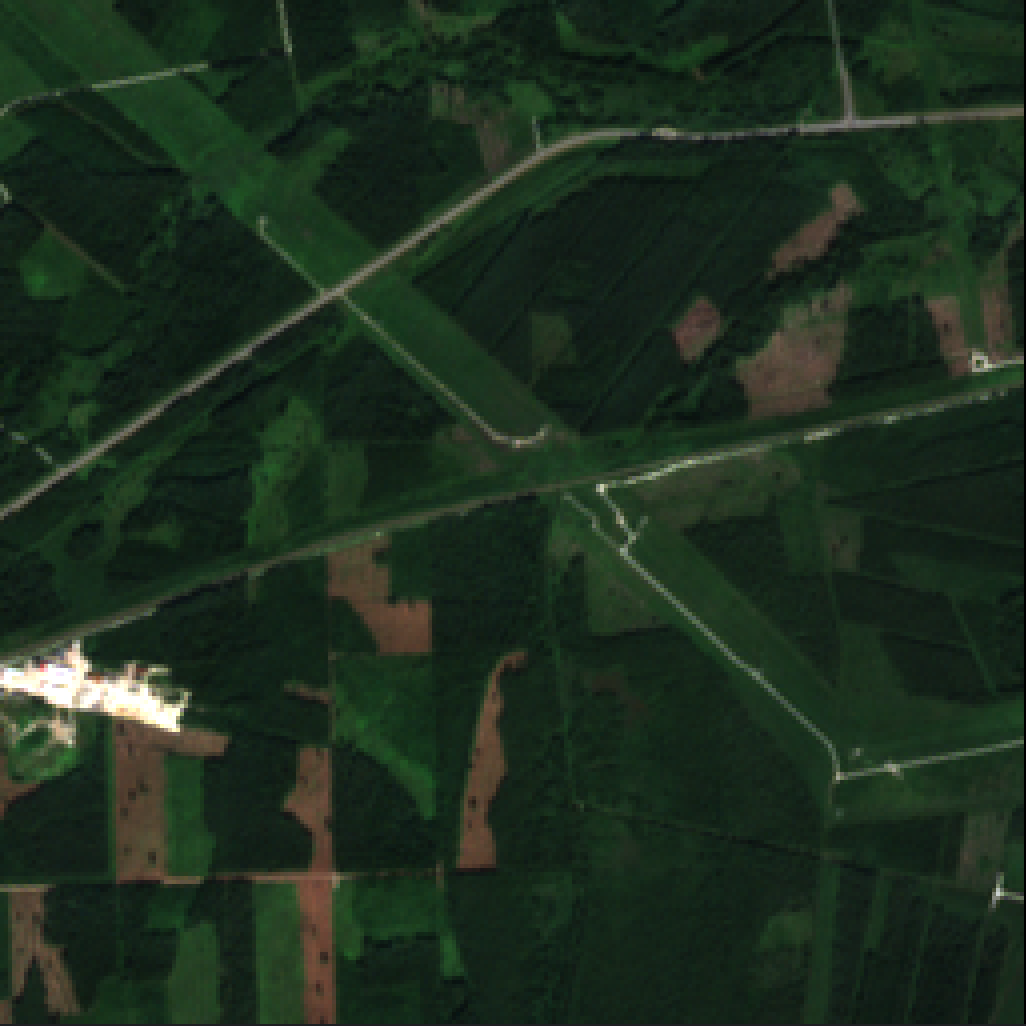
\includegraphics[width=0.5\textwidth]{figures/andmestik/lr_3308099_TCI.png}
    %    \caption{} % Leave caption empty to automatically label this subfigure as (b)
    %    \label{fig:satellite_example}
    %\end{subfigure}

    \caption{Näidis ühe lageraie päringust saadud ümbrusest (a) ja satelliitpildist (b).}
    \label{fig:sidebyside_teatis_sat_img}
\end{figure}

Magistritöö peamiseks uurimisküsimuseks on, kas ja kuidas on võimalik kasutada väheste näidete (\textit{Few-Shot}) põhist alusmudelit. Väikese valimi puhul on aga vaja eriti täpseid andmeid millelt õppida. Nagu eelnevalt mainitud siis metsaregistrist saadud andmed ei ole piisavalt täpsed, et neid otse kasutada alusmudeli treenimisel metsaraie tuvastamiseks, mis on illustreeritud Joonisel \ref{fig:sidebyside_teatis_sat_img}. Esiteks on küsimus, kui kaua pärast raieteatise kehtima hakkamist metsa raiuti, kui üldse raiuti, ja teiseks esineb raieid, mis ei püsi rangelt metsajaotiste piirides. Lisaks paistab raiutud mets raiutud metsana erineva perioodi vältelt sõltuvalt raie aastaajast -- suvisel ajal muutub raiutud ala kiiremini roheliseks.

Seetõttu lisandusid uurimistöösse andmete täiendava töötlemise ja maskimise etapid, kus andmed käiakse käsitsi läbi, kasutades registri andmeid maski põhjana. Ajalise piirangu tõttu pidi tegema alamvalimi. Et saada Eesti metsade kohta üldisemaid näiteid kasutati selleks KMeans klasterdamise meetodit, et jagada metsad omakorda kahte erinevasse klassi okas- ja lehtpuud. Eesmärgiks oli koguda kokku 100 raiet ja nende ümbrust, et luua piisavalt andmeid, mille pealt mudelit treenida. Kui peaks juhtuma et mõni pilt pole kõlbulik, siis valitakse samast alamvalimist uus lageraie piirkond. Valitud alad on toodud Joonisel \ref{fig:kmeans}. 

\begin{figure}[H]
    \centering
    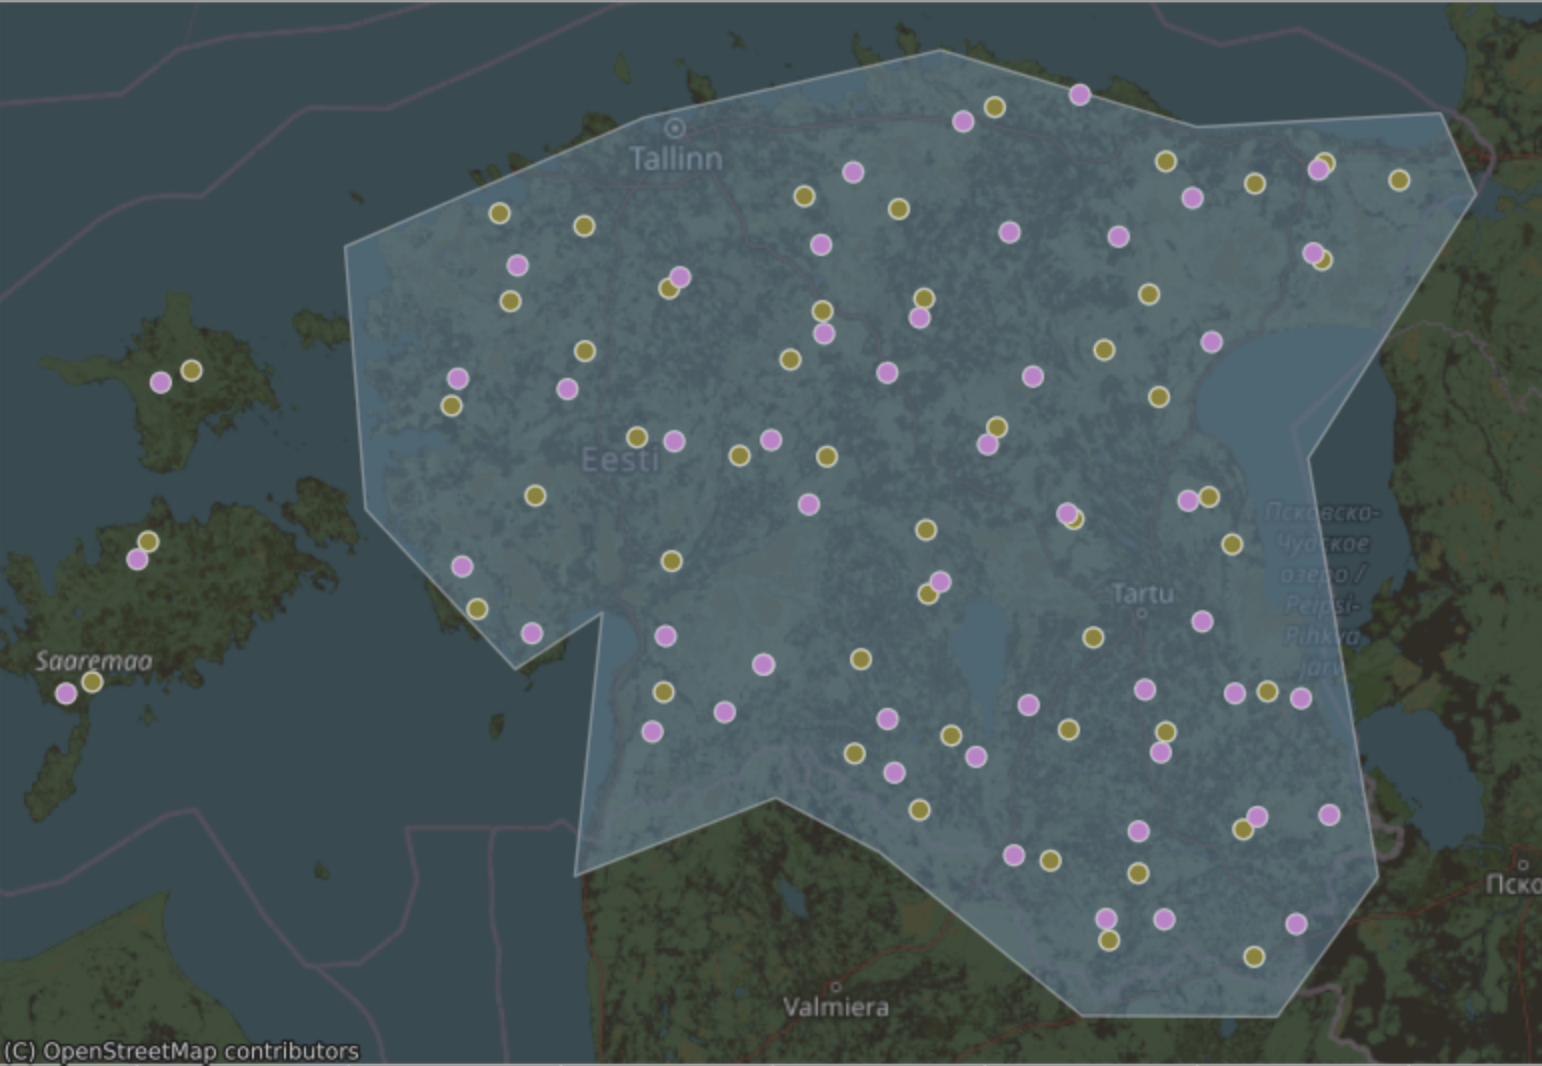
\includegraphics[width=.9\textwidth]{figures/andmestik/kmeansmap.png}
    \caption{KMeans klasterdamise tulemus, 100 raie ümbrust leht- või okaspuudega}
    \label{fig:kmeans}
\end{figure}


Peale selle etapi lõppu, kus on loodud 100 raie ümbrust polügoonidena. Edasi kirjeldatakse lahti sammud, välja toodud Joonisel \ref{fig:terveflow}, et saada nendega seonduvad satelliitpildid.

Töös kasutatud andmestik koosneb 15. lageraie piirkonnast. Alljärgnevalt on tabel mis toob välja lageraie ID ja jäädvustus kuupäeva.
\bigskip


\begin{longtable}{ll}
    \hline
    \textbf{Lageraie ID} & \textbf{Jäädvustus kuupäev} \\
    \hline
        226703.0 & 2023/08/04 \\
        3464763.0 & 2022/10/13 \\
        3310419.0 & 2020/10/11 \\
        3542301.0 & 2023/11/13 \\
        3307283.0 & 2020/09/16 \\
        204935.0 & 2022/09/26 \\
        3543143.0 & 2023/11/07 \\
        3536617.0 & 2023/08/28 \\
        3468479.0 & 2022/10/04 \\
        3453239.0 & 2022/08/23 \\
        \hline
\end{longtable}


Kuna andmete päring ja töötlemine nõudis suurt arvutus- ja salvestusressurssi,
algas töö ühe üksiku lageraie piirkonna ja selle vahetu ümbruse salvestamisega
ühte .shp-vormingus vektorfaili. Edasiste testide käigus selgus, et optimaalne
lähenemine hõlmab 10--15 lageraie ala ning nende ümbruste sõltumatut päringut ja
salvestamist eraldi shape-failidena. Selle põhjal viidi läbi järgnev töölõikude
jadastik:
\begin{enumerate}[topsep=1pt,itemsep=1ex,partopsep=1ex,parsep=1ex]

\item \textbf{Shape-failide loomine ja kokkuliitmine}\newline
Iga lageraie piirkonna ja selle vahetu
ümbruse (buffer) geomeetria päriti riiklikust puistu andmebaasist ja salvestati
iseseisvatesse shapefile'idesse. Selle lähenemise eeliseks oli võimalus
vajalikke alasid hõlpsalt lisada või eemaldada ilma terve andmestiku
ümberlaadimiseta. Paremaks haldamiseks ja analüütiliseks töötluseks liideti kõik
eraldi genereeritud shapefile'id  tervikusse, mis võimaldas
vektorandmete ühtlustatud töötlemist järgmistes etappides.

\item \textbf{Piltide päring Sentinel-2 andmebaasist} \newline
Iga shape-failiga määratletud lageraie
ala serva genereeriti puhvrina ristkülikukujuline ``kast'' (bounding box), mis
täielikult kataks huvipakkuva piirkonna. Selle kasti geomeetria alusel loodi
päring Sentinel-2 metadatebaasist, eesmärgiga leida piirkonnale vastav optiline
satelliitpilt. Päringule lisati järgmised piirangud:

\begin{enumerate}

\item \textbf{Ajapiirang}: pildistamise kuupäev peab jääma lageraie teadmisest alates kuni 40
päeva jooksul, tagamaks muutuste jälgitavuse tuvastamise võimalikult värskel
materjalil.

\item \textbf{Pilvekatte piirang}: pilt valiti vastavalt väikseimale keskmisele pilvekattele,
et maksimeerida nähtavust ja andmete kvaliteeti.
\end{enumerate}

Kui sobiliku satelliitpilti nimetatud tingimustel ei leitud,
laiendati ajavahemikku ning tõsteti lubatavat pilvkatte protsenti kuni eelnevalt
määratud lävendini. Sel juhul, kui sobivat pildistust ikkagi ei tuvastatud,
alustati protsess uuesti järgmise lageraie piirkonnaga samas klastris, et tagada
piisav andmepunktide hulk analüüsi teostamiseks.

\item \textbf{Andmete allalaadimine ja eeltöötlus} \newline
 Sobiva Sentinel-2 toote puhul laeti
vastav .SAFE kataloog alla. Sentineli toode sisaldab üheskoos nii optilisi riba-
(band) kui ka metadatastruktuure, mis on vajalikud edasiseks detailseks
analüüsiks. Eriti olulised on:

\begin{enumerate}
\item \textbf{Spektraalsed ribad} (sh paindliku dünaamikaga B02--B12 ja veespetsiifilised B8,
B8A), mis võimaldavad eristada metsaobjekte ja maapinnanähtusi.

\item \textbf{Pilve- ja lumeindeksiriba (B10)}, mis lihtsustab pilvisuse automaatset
tuvastamist ning tagab eeltöötlemisel täpsema piirkondliku pilvete kaardistamise.
\end{enumerate}

\item \textbf{Atmosfääriline korrektsioon ja lõikamine} \newline
Kõigilt valitud optilistelt ribadelt
viidi läbi atmosfääriline korrektsioon, kasutades Sentinel-2 töötlemise
standardalgoritmi (Sen2Cor või QGIS'i lahtise lähtekoodiga moodul), et eemaldada
atmosfäärist tulenevad häired (nt aerosoolid, gaasiline neeldumine). Pärast
korrektsiooni genereeriti rasterfailide (level-2A) baasil täpsed TIFF-vormingus
pildid, kus iga kanal (band) on salvestatud eraldi kihina, säilitades
kooskõlastatud ruumilist ja spektraalset täpsust.

\item \textbf{Huvipiirkondade täpne väljavõtmine} \newline
Lõpuks lõigati korrektsiooni läbinud
piltidelt välja eelnevalt genereeritud kastide ulatuses täpsed rasterfragmendid,
et töödelda vaid huvipakkuvaid alasid. Selline meetod tagab, et iga lageraie
objekt ja selle ümbrus on rasterandmes täpselt isoleeritud, mis lihtsustab
edasist masinõppe- ja analüüsitöötlust. Lõppfailid salvestati
georefereeritud GeoTIFF-idena, mis toetavad mitmetasandilisi kanalivaateid
ja on integreeritavad GIS-keskkondadesse.

\end{enumerate}
Käesolev töövoog võimaldas optimeerida andmekäitluse ressursikasutust, tagada
piltide kõrge kvaliteet ning kindlustada, et iga lageraie piirkonnast on saadud
piisav hulk informatsiooni edaspidiseks statistiliseks ja mudelipõhisteks
analüüsideks.


\begin{figure}[H]
    \centering
    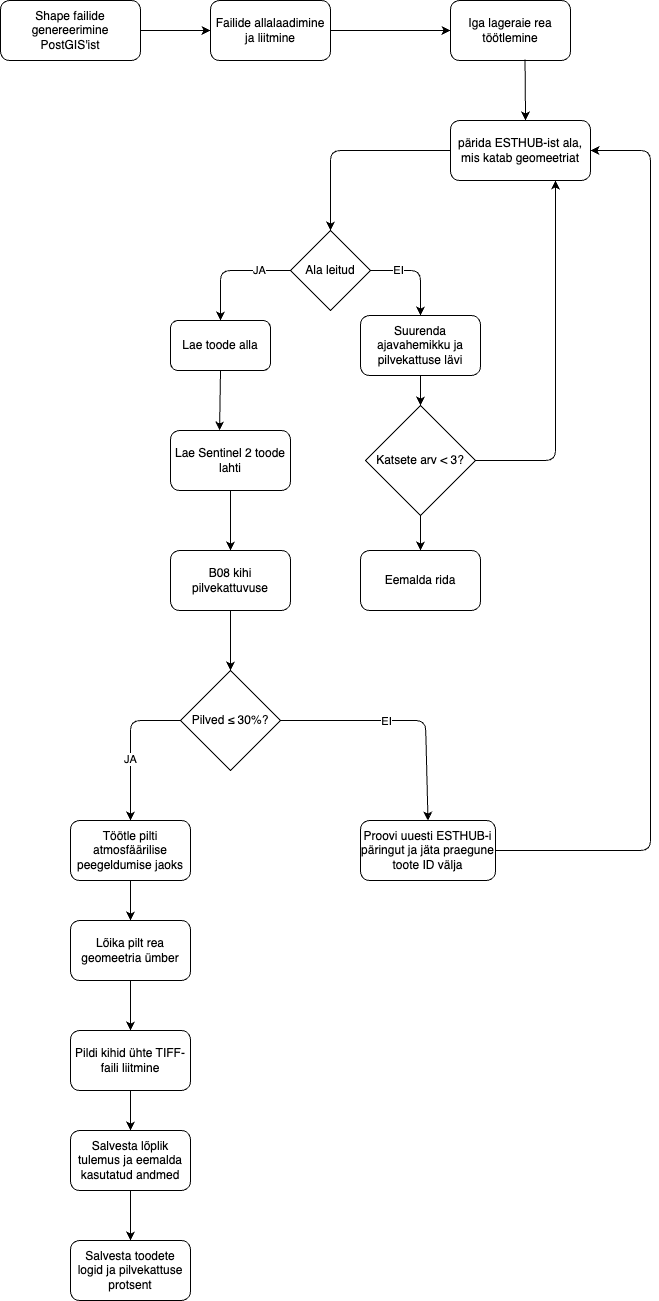
\includegraphics[width=.8\textwidth]{figures/andmestik/andmete_voog.drawio.png}
    \caption{Andmestiku loomise töövoog}
    \label{fig:terveflow}
\end{figure}


\subsection{Raie piirkonna maskide loomine}
Selles peatükis käsitletakse andmete maskimist, kuna metsaregistrist saadud andmed pole piisavalt täpsed, et neid otse masinõppes kasutada, siis sai loodud sammud, et andmeid täpsemaks muuta. Terviklik dokument on töö lisade hulgas.

Eesmärk oli luua dokument, mis aitaks kõigil kasutajatel luua vektormaske kasutades selleks enne mainitud QGISi tarkvara. Selleks et anda parem hinnang pildil olevatele aladele on kasutusel võetud kihid. Kaks peamist kihti on:
\begin{itemize}[topsep=1pt,itemsep=1ex,partopsep=1ex,parsep=1ex]
    \item \textbf{Metsateatised} --- andmed, mis on saadud riiklikust metsaregistrist ja sisaldavad teavet metsateatise esitamise kuupäeva, metsateatise menetlemise kuupäeva, metsateatise kehtivuse alguskuupäeva ja metsateatise kehtivuse lõppkuupäeva kohta. Selle info abil saab kindlaks teha, kas üldse on vaja märgendada antud piirkonda.
    \item \textbf{Ortofotod} --- on kõrge eraldusvõimega õhust tehtud fotod, mis on georefereeritud ja millel on täpselt määratletud koordinaadid. Ortofotod võimaldavad täpset analüüsi ja hindamist, et tuvastada metsade seisundit ja muudatusi. Ortofotosid tehakse harvemini kui näiteks Sentinel-2 satelliidipilte ja mitte alati üle terve Eesti, kuid need on vajalikud, et saada täpsemat teavet metsade seisundi kohta. Ortofotod on saadaval erinevates spektraalsetes ribades, sealhulgas nähtavas ja infrapunases spektris, mis võimaldab analüüsida erinevaid maapinna omadusi. Käesolevas töös kasutati nii RGB kui ka CIR-NIR ortofotosid. 
\end{itemize}

Teiseks on dokumendis toodud välja juhtnöörid ja soovitused, mida peaks järgima
maskide loomisel. Järgnevalt on välja toodud mõned näidised, mis illustreerivad ortofotode ja Sentinel-2 piltide erinevusi, seega on tähtis, et orotfotosid kautatakse juhtnööridena aga mitte põhitõena. Masinõppes kasutatavate andmete kvaliteet antud uurimistöös mängib suurt rolli, seega kui maskide loomise käigus tekkis kahtlusi klassi tuvastamises, siis jäeti need alad alati välja.

Joonisel \ref{fig:sent_mask_naidis}, Joonisel \ref{fig:orto_mask_naidis} ja Joonisel \ref{fig:orto_nir_mask_naidis} on välja toodud näidised, mis illustreerivad Sentinel-2 saadud pilti ja selle sama piirkonna ortofotosid. NGR värvi tõlgendused on toodud välja varasemas Peatükis \ref{chapter:taust} Tabelis \ref{tab:NGR_kasutus}. Oranžiga on välja toodud piirkond, mille Sentinel-2 sateliidipildi järgi peaks märkima lageraieks, RGB ortofoto samuti viitab sellele. NGR pildil on ka näha tsüaan tooni, mis viitab sellele, et seal peaks olema mulda, ehk suure tõenäosusega võib seal olla lageraie. Siinjuhul peab meeles pidama ka, et uurimistöös kasutatud ortofotode ja Sentinel-2 piltide vahel on ajaline erinevus ja olgugi, et ortofotol on selgesti oranžis kastis kaks lageraiet, siis Sentinel-2 pildi järgi saab märkida ainult ühe neist lageraieks. Metsa näidis on toodud välja rohelise kastiga, millel on kõigil kolmel pildil suuresti ühtlane kattuvus. Eraldi on piltidel kollase kastiga välja toodud heinamaa piirkond. Heinamaad ja põllumaad on alad, mis satelliitpildilt ja RGB ortofoto võivad põgusal vaatamisel tunduda lageraie alana, kuna seal puid ei kasva, aga kui vaadata lähemalt NGR pilti, siis on näha, et seal on vähem mullale viitavat tsüaan tooni, millest võib järeldada, et seal võiks hoopis põld asuda.

\begin{figure}[H]
    \centering
    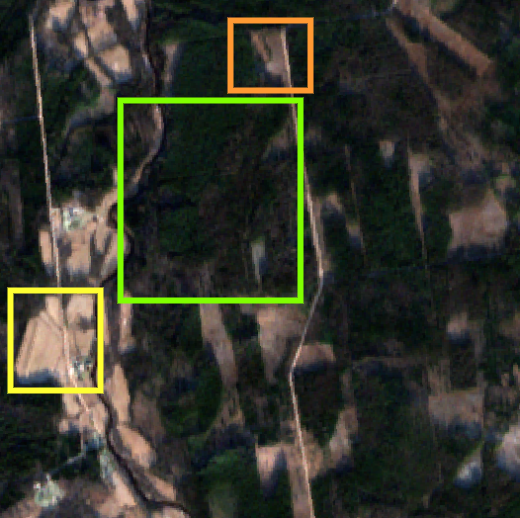
\includegraphics[width=.6\textwidth]{figures/andmestik/tuvastamis_sent2_naidis.drawio.png}
    \caption{Sentinel-2 RGB näidis}
    \label{fig:sent_mask_naidis}
\end{figure}

\begin{figure}[H]
    \centering
    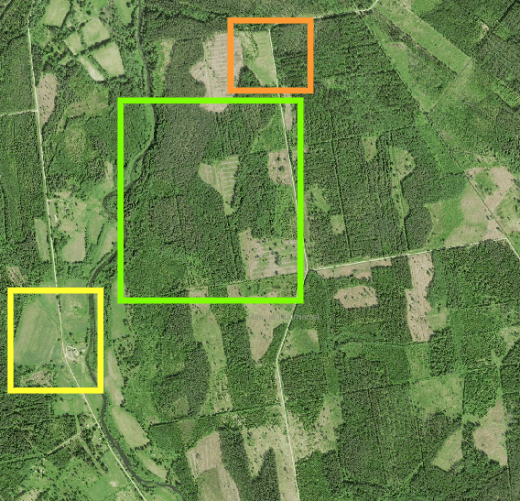
\includegraphics[width=.6\textwidth]{figures/andmestik/tuvastamis_orto_naidis.drawio.png}
    \caption{RGB ortofoto näidis}
    \label{fig:orto_mask_naidis}
\end{figure}

\begin{figure}[H]
    \centering
    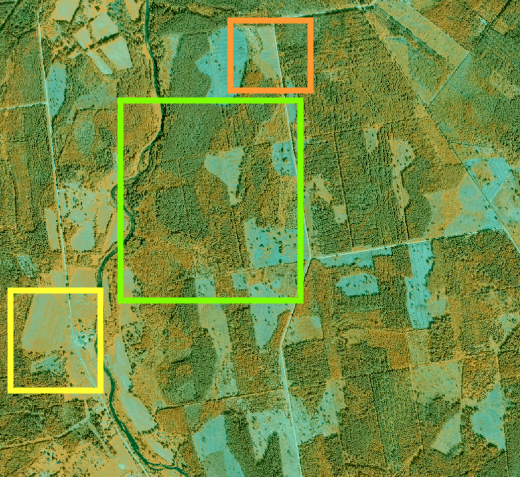
\includegraphics[width=.6\textwidth]{figures/andmestik/tuvastamis_orto_nir_naidis.drawio.png}
    \caption{CIR-NGR ortofoto näidis}
    \label{fig:orto_nir_mask_naidis}
\end{figure}
